% Changing book to article will make the footers match on each page,
% rather than alternate every other.
%
% Note that the article class does not have chapters.
\documentclass[letterpaper,10pt,twoside,twocolumn,openany]{book}

% Use babel or polyglossia to automatically redefine macros for terms
% Armor Class, Level, etc...
% Default output is in English; captions are located in lib/dndstring-captions.sty.
% If no captions exist for a language, English will be used.
%1. To load a language with babel:
%	\usepackage[<lang>]{babel}
%2. To load a language with polyglossia:
%	\usepackage{polyglossia}
%	\setdefaultlanguage{<lang>}
\usepackage[english]{babel}
%usepackage[italian]{babel}
% For further options (multilanguage documents, hypenations, language environments...)
% please refer to babel/polyglossia's documentation.

\usepackage[utf8]{inputenc}
\usepackage{lipsum}
\usepackage{listings}
\usepackage{hyperref}

% dnd package options 
% bg-full   : Default option. Use paper background and fancy footer.
% bg-print  : Use fancy footer but not background.
% bg-none   : No paper background and plain footer.
% justified : Use full justification for text layout instead of ragged right.
\usepackage{dnd}

\lstset{%
  basicstyle=\ttfamily,
  language=[LaTeX]{TeX},
}

% Start document
\begin{document}

% Your content goes here

% Comment this out if you're using the article class.
\chapter{File ARchive Kit (FARK)\tiny{met.no, 2018}}

\section{Introduction}
The process of generating {\bf verification results} by co-locating {\bf observation} and {\bf model data}, 
typically requires 200 pieces of information.
The FARK system provides a web-interface \url{http://fark.met.no} for the user to specify this information and
organize the regular production of verification result.

\begin{quotebox}
   Use FARK if you need {\bf regular production} of {\bf verification results} 
   and don't want to spend your time writing scripts.
\end{quotebox}

\subsection{FARK production}

FARK first generates {\bf indexed lists} of the {\bf NetCDF} model files 
and {\bf BUFR} observation files that will be used in the verification.
\begin{quotebox}
File indexes are usually sorted by the epoch-time.
\end{quotebox}
A basic description of the NetCDF and BUFR file formats is available in the \hyperlink{appendix}{{\em appendix}}.

Next, model fields are interpolated to relevant observation locations and time.
This co-located data is written to a {\bf table file} according to the specifications in a {\bf plotting script}.

Finally, the {\bf plotting script} produces the {\bf verification plots}.

\begin{quotebox}
Verification results are found under:
\href{/lustre/storeA/project/nwp/fark/.}{\lstinline!/lustre/storeA/project/nwp/fark!}
\end{quotebox}

\section{Web interface}
All information necessary to generate verification results can
be put into the FARK web interface.
The web interface contains buttons designed to make it easier for the
user to provide this information.

\subsection{Buttons}

\begin{dndtable}[cX][DmgCoral]
  \textbf{Button} & \textbf{Description} \\
  \raisebox{-0.2\height}{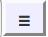
\includegraphics[height=13pt]{server.jpg}}& show alternatives\\
  \raisebox{-0.2\height}{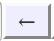
\includegraphics[height=13pt]{left.jpg}}  & move information\\
  \raisebox{-0.2\height}{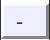
\includegraphics[height=13pt]{minus.jpg}} & delete table entry\\
  \raisebox{-0.2\height}{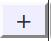
\includegraphics[height=13pt]{plus.jpg}}  & add table entry\\
  \raisebox{-0.2\height}{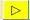
\includegraphics[height=13pt]{test.jpg}}  & test process\\
  \raisebox{-0.2\height}{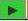
\includegraphics[height=13pt]{run.jpg}}   & start process\\
  \raisebox{-0.2\height}{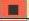
\includegraphics[height=13pt]{stop.jpg}}  & stop process\\
  \raisebox{-0.2\height}{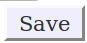
\includegraphics[height=13pt]{save.jpg}}  & save setup to server
\end{dndtable}

The web interface is further divided into the following tabs: \lstinline!Model!, \lstinline!Observation!, \lstinline!Colocation!, 
\lstinline!Plot! and \lstinline!Auto!.

\begin{quotebox}
Press the ``tab title'' to reload data from server.
\end{quotebox}

\subsection{Model tab}

\begin{paperbox}{Model tab}
  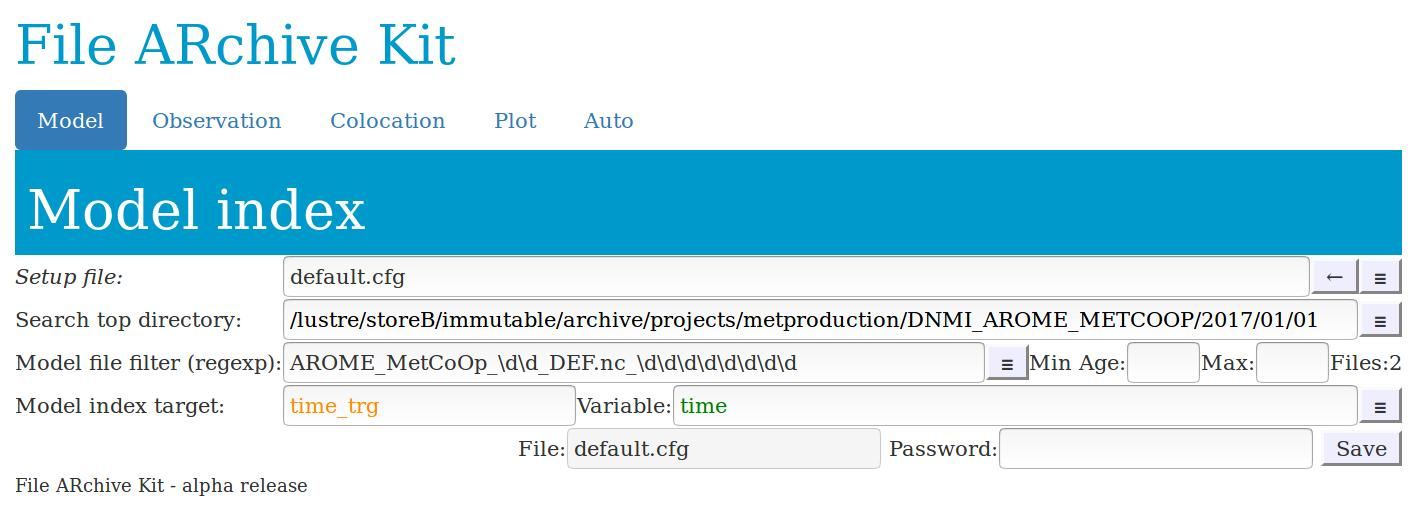
\includegraphics[width=\columnwidth]{fark_model.jpg}
\end{paperbox}
In this tab you specify which \hyperlink{netcdf}{NetCDF} model files to index and which variable to use when sorting the  {\bf model index}.
The index sorting variable is given a {\bf model index target} name.

\begin{quotebox}
  A {\bf target} name is a 'short name' used to
  represent the model variable or observation 
  parameter.
\end{quotebox}
When a model file is being indexed, FARK will pre-scan the range of the variables with small array size.

\subsection{Observation tab}
\begin{paperbox}{Observation tab}
  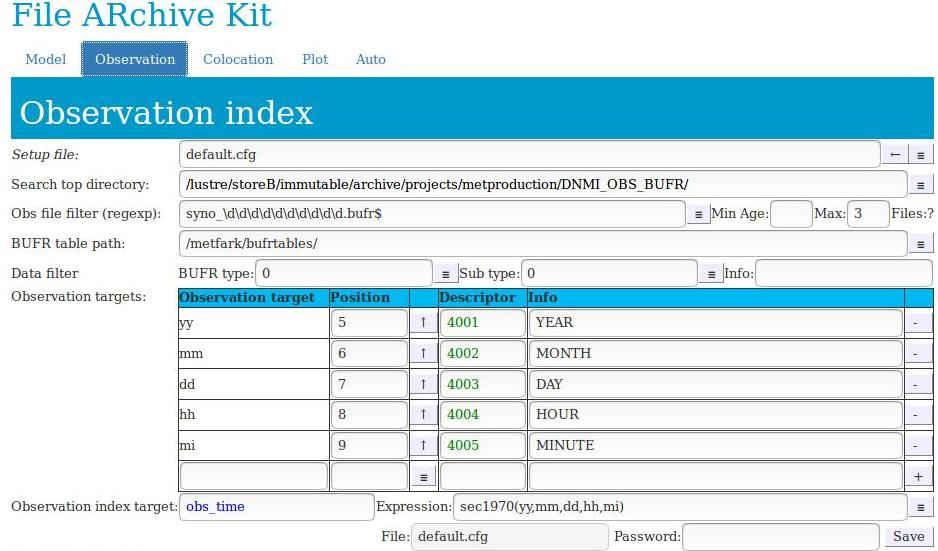
\includegraphics[width=\columnwidth]{fark_obs.jpg}
\end{paperbox}
Here you specify which \hyperlink{bufr}{BUFR} observation files to index, and 
the {\bf expression} used to sort the {\bf observation index}.
The index expression is assigned a {\bf target} name. The user must also define the {\bf observation targets} that are used in the index expression. The observation targets point to specific positions in the \hyperlink{sequence}{BUFR sequence}.
\begin{quotebox}
Files match if their index target range overlap.
\end{quotebox}

\subsection{Colocation tab}
This is where you specify how the model and 
observation data should be matched.
The colocation tab contains several tables.

\subsubsection{Model targets table}
\begin{paperbox}{Model targets table}
  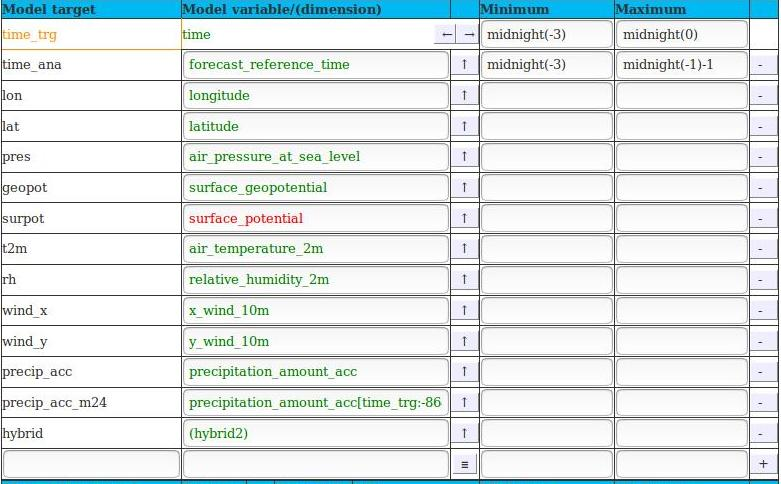
\includegraphics[width=\columnwidth]{coloc_model.jpg}
\end{paperbox}
The {\bf model targets} table lists model variables and their target names.
The (saved) {\bf model index} target name is listed first.
\begin{quotebox}
  Variables in red are not in the scanned model file.
\end{quotebox}
The {\bf model target} can also be a {\bf dimension}. 
In this case enter the dimension name surrounded by brackets instead of a variable name,
for instance \lstinline!(ensemble_member)!.
\begin{paperbox}{Model variable offset}
  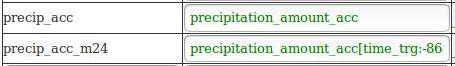
\includegraphics[width=\columnwidth]{offset.jpg}
\end{paperbox}
If you want a model variable, say 24 hours earlier than the observation time, you can use an {\bf offset}.
The square brackets added after the variable name should contain the 
name of the model target that should be offset and the offset amount (separated by colon).
In this example model target \lstinline!precip_acc_m24! contains the accumulated precipitation 24 
hours before the target \lstinline!precip_acc!.
\hyperlink{matching}{\em Matching rules}) should not be defined for offset model targets .

\subsubsection{Observation targets table}
\begin{paperbox}{Observation targets table}
  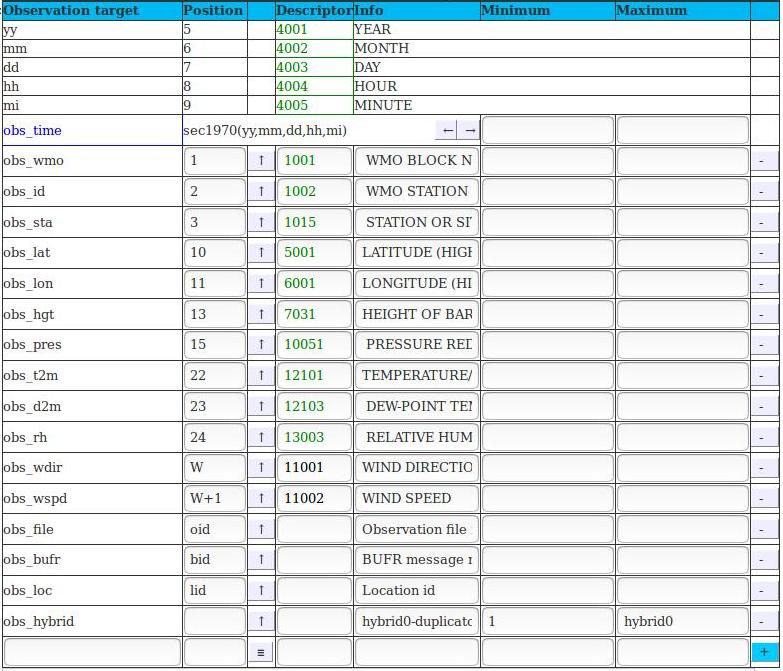
\includegraphics[width=\columnwidth]{coloc_obs.jpg}
\end{paperbox}
In the {\bf observation targets} table the user can specify observation targets in the BUFR sequence.
The targets already defined in the (saved) {\bf observation index} are listed first. 
Additional observation targets needed to match the observation with the model fields are added here.

\subsubsection{Position variables}
In the example above \lstinline!obs_wdir! uses a {\bf position variable}, \lstinline!W! 
instead of a number. 
The reason for this is that the wind speed happens to appear after a \hyperlink{delayed}{\em delayed replicator} 
in the BUFR sequence.
The FARK system will search the BUFR sequence for the specified descriptor, \lstinline!11001!,
and assign the corresponding position to the {\bf position variable},  \lstinline!W!. 
The {\bf position variable} can be used in the position expressions of later observation targets,
as we see in the example with \lstinline!obs_wspd! with the position expression \lstinline!W+1!.
FARK will repeat the search for position variables until the end of the BUFR message, giving a new location for every match found.

\begin{quotebox}
   Use {\bf position variables} when you process radiosonde TEMP BUFR messages.
\end{quotebox}

If only the descriptor is specified, the system will search the BUFR sequence 
for the next entry with the given descriptor.

\subsubsection{Internal variables}
Internal variables are indicated as position variables in the position field,
without any descriptor.
\begin{dndtable}[cX][DmgCoral]
  \textbf{Position} & \textbf{Description} \\
  mid &  model file index position\\
  oid &  observation file index position \\
  bid &  BUFR message number \\
  sid &  observation number in message \\
  lid &  location number in message
\end{dndtable}

\begin{quotebox}
A location is identified using {\bf oid}, {\bf bid} and {\bf lid}.
\end{quotebox}

\subsubsection{Duplicate location}
If you want to compare the same observation location to several model fields, for instance different ensemble members,
you need to duplicate the observation location.
In this case you specify the min and max values and not the position nor descriptor
(the max value may be a model dimension).

\begin{quotebox}
   Duplicate locations if you need to process multiple {\bf model ensemble members}.
\end{quotebox}
The observation target \lstinline!obs_hybrid! in the example above is an example of location duplication.
The target \lstinline!obs_hybrid! takes the value of the duplication index, i.e. \lstinline!1,2,3,...,hybrid0!.

\hypertarget{matching}{}
\subsubsection{Match rules table}
The {\bf match rules} table specifies how the model targets should match the
observation targets. 
\begin{paperbox}{Match rules table}
  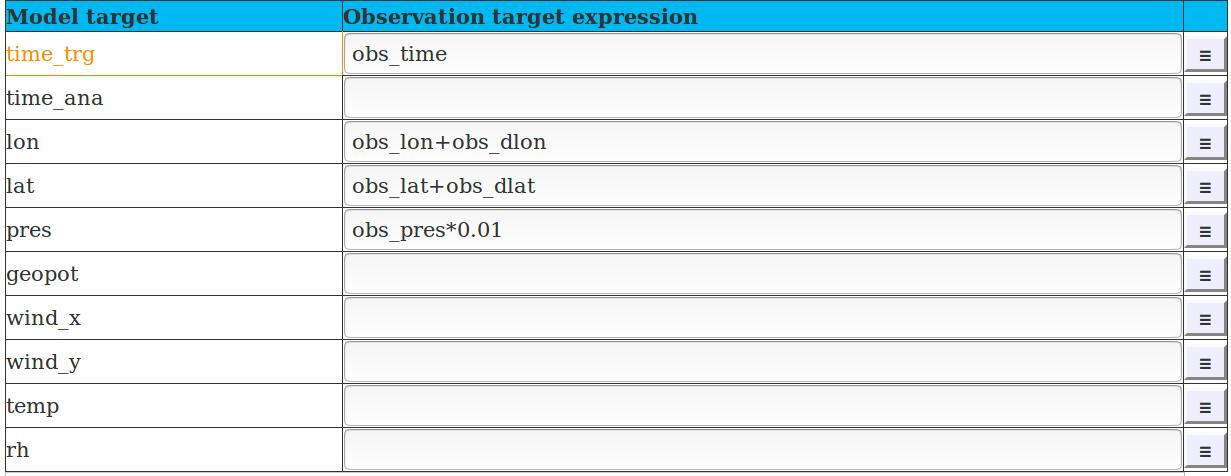
\includegraphics[width=\columnwidth]{coloc_match.jpg}
\end{paperbox}
Model targets with blank observation target expressions are not used for matching.
If insufficient matching rules are specified so that FARK can not determine how to
interpolate a dimension used by a model target, FARK will average over that dimension (if it is small).

\begin{quotebox}
A location is discarded if a match rule has a target that is undefined.
\end{quotebox}

\hypertarget{default}{}
\subsubsection{Default table}
The {\bf default} table is only visible if the observation index file has been set to \lstinline!<none>!.
The default table specifies how the model targets should match default values.
\begin{paperbox}{Default table}
  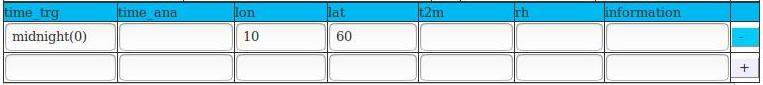
\includegraphics[width=\columnwidth]{default.jpg}
\end{paperbox}

\subsubsection{filters}

Co-location takes a lot of computer resources, and it is therefore a good strategy
to filter out unwanted data as early as possible in the data processing.
The plot log in the \lstinline!Auto tab! contains summaries of how different filters and the quality control removed data.

\begin{paperbox}{Model target filter}
  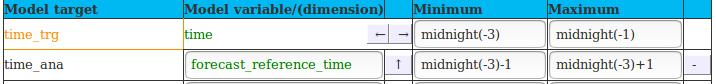
\includegraphics[width=\columnwidth]{filter_minmax.jpg}
\end{paperbox}
If a model target has {\bf min} and {\bf max} limits that are outside the pre-scanned range, 
the model file will immediately be rejected. Below is an example of the resulting plot log summary.
\begin{paperbox}{Plot log (model file filter)}
  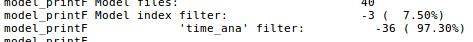
\includegraphics[width=\columnwidth]{filter_minmaxlog.jpg}
\end{paperbox}

The observation {\bf min} and {\bf max} filters are applied as the BUFR messages are read from the observation file.

The {\bf observation filter} expression is applied to all locations in a BUFR message at once,
and has functions like
\begin{lstlisting}
   msgclosest(obs_pres*0.01,1000,500)
\end{lstlisting}
that selects the locations with the expression, \lstinline!obs_pres*0.01!, closest to the given list, \lstinline!1000,500!.
\begin{quotebox}
  The {\bf observation filter} expression can only be based on observation targets.
\end{quotebox}

The model {\bf min} and {\bf max} filters are re-applied immediately after the corresponding 
model field has been interpolated to the observation location.

The {\bf location filter} expression is applied when all relevant model fields have been interpolated to the observation location.
This is the most expensive filter in terms of computer resources.

There is a debug option available for testing the built in filter functions.
The debug expression can not accept any targets.
Note that ``blank'' returns zero.

\begin{quotebox}
  A location is rejected if a filter expression returns 0.
\end{quotebox}


\subsection{Plot tab}

\begin{paperbox}{Plot tab}
  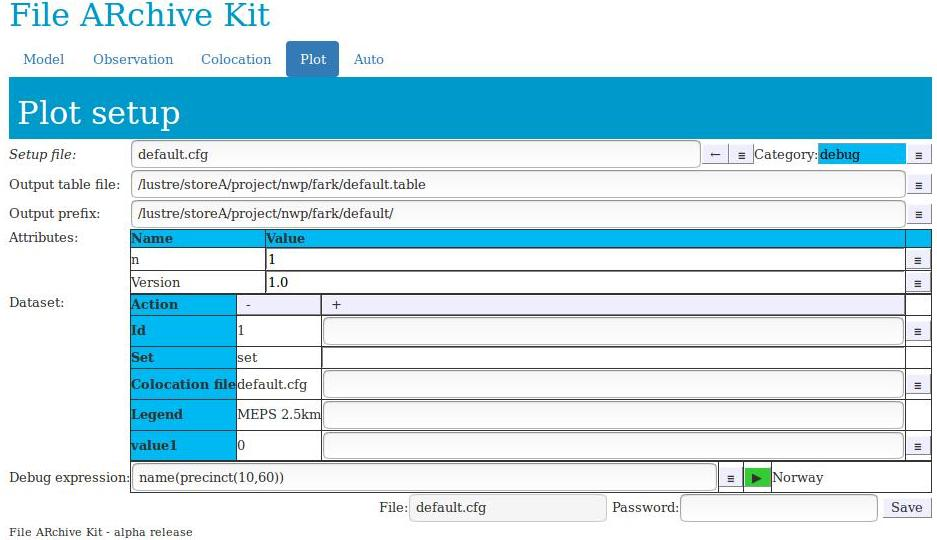
\includegraphics[width=\columnwidth]{fark_plot.jpg}
\end{paperbox}

This is where you provide information requested by the plotting script.
The user chooses plotting script in the \lstinline!Category! field.

Verification results are placed on disk according to the \lstinline!Output table file! and \lstinline!Output prefix! paths.
Use \lstinline!YY MM DD HH MI! as wildcards in the output paths.

There are two tables in the plot tab. 
The {\bf Attributes} table allows the user to specify attributes that apply for all the data,
for instance titles, units and labels.
Some attributes can only have fixed values, indicated by an action button
 \raisebox{-0.2\height}{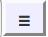
\includegraphics[height=13pt]{server.jpg}}.
Special attributes can be used to enumerate other attributes and columns.

A plotting script can compare different colocation datasets.
The {\bf Dataset} table assigns every dataset an \lstinline!Id!, \lstinline!Colocation file! and 
\lstinline!legend!, along with the columns requested by the plotting script.

\subsection{Auto tab}
\begin{paperbox}{Auto tab}
  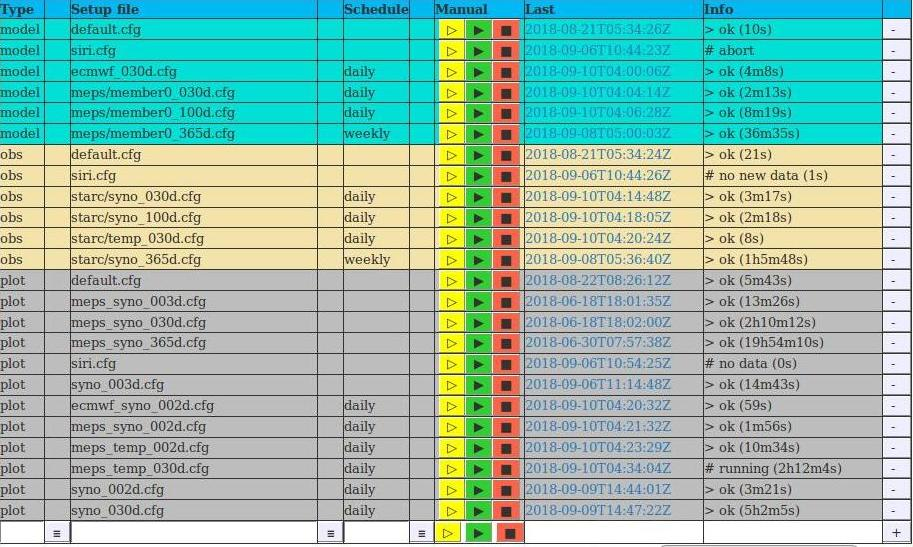
\includegraphics[width=\columnwidth]{auto.jpg}
\end{paperbox}

This is where you tell the computer to actually do some work.
Available types of jobs are:
\begin{dndtable}[cX][DmgCoral]
 {\bf Type} & {\bf Description} \\
 model & maintain model index file, \\
 obs & maintain observation index file, \\
 coloc & {\em debugging for advanced users,} \\
 plot & generate verification products.
\end{dndtable}
Each job can be executed manually or according to a schedule.

\begin{quotebox}
  The \lstinline!Last! column has links to log files from the
  last {\bf successful} and {\bf un-successful} runs.
\end{quotebox}

%The task configuration can be {\bf tested} manually by pressing 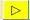
\includegraphics[height=13pt]{test.jpg}. 
%Tasks can be {\bf executed} manually by pressing 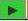
\includegraphics[height=13pt]{run.jpg}.
%A running task can be {\bf stopped} manually by pressing 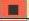
\includegraphics[height=13pt]{stop.jpg}.

\section{HOW TO...}

\subsection{...create a model index}
Change focus to the ``Model'' tab.
\subsubsection{1. Make sure index does not exist}
Enter the name of your new index in the \lstinline!setup file:! field, for instance \lstinline!test.cfg!,
and press  \raisebox{-0.2\height}{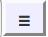
\includegraphics[height=13pt]{server.jpg}} next to the field.
\begin{paperbox}{Model tab}
  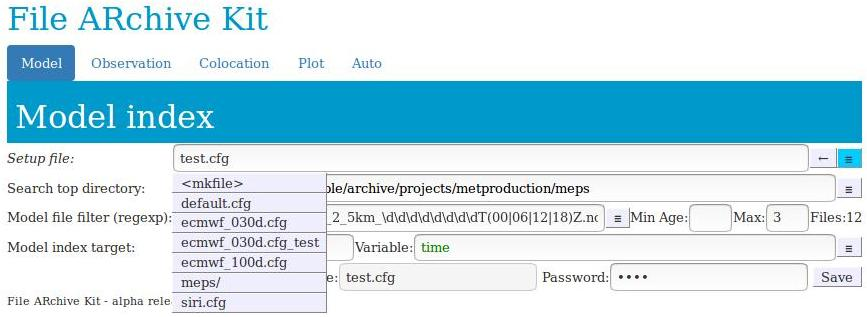
\includegraphics[width=\columnwidth]{how_mod.jpg}
\end{paperbox}
If your options include \lstinline!<mkfile>! then the index does not exist.
If the index already exists, the index setup will be loaded automatically.
In this case press \lstinline!<rmfile>! to delete the existing index.
Remember to use the correct password when changing or deleting an existing index.
Finally, press \raisebox{-0.2\height}{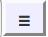
\includegraphics[height=13pt]{server.jpg}} again and ``forget'' the index on your client by pressing  \lstinline!<fgfile>!.
\subsubsection{2. Find a suitable index to copy}
Enter the name of the index you wish to copy in the \lstinline!setup file:! field.
You may press \raisebox{-0.2\height}{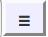
\includegraphics[height=13pt]{server.jpg}} to navigate.
The index setup will be loaded automatically when an existing index is specified.
\subsubsection{3. Create new index setup}
Enter the name of the new and non-existing index you wish to create in the \lstinline!setup file:! field.
Select the password that has to provided when changing or deleting the new index.
Press {\raisebox{-0.2\height}{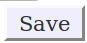
\includegraphics[height=13pt]{save.jpg}} to create the index setup on the server.
\subsubsection{4. Edit the new index setup}
Edit the index setup fields.
You may press \raisebox{-0.2\height}{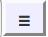
\includegraphics[height=13pt]{server.jpg}} next to
\lstinline!Model file filter(regexp)! to select which model file to scan.
Variables in the scanned file appear as
relevant options to other fields (when pressing \raisebox{-0.2\height}{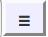
\includegraphics[height=13pt]{server.jpg}}),
for instance  \lstinline!Variable:!.
When you are satisfied, press \raisebox{-0.2\height}{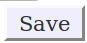
\includegraphics[height=13pt]{save.jpg}} to save your settings.
\subsubsection{5. Create the model index}
Switch to the \lstinline!Auto! tab.
The last row in the table allows you to enter new jobs.
Select the \lstinline!model! type, and press \raisebox{-0.2\height}{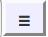
\includegraphics[height=13pt]{server.jpg}} next to \lstinline!Setup file!.
\begin{paperbox}{Auto tab}
  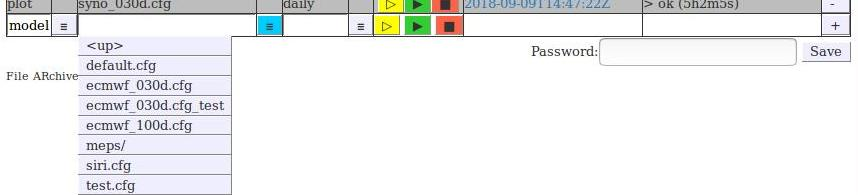
\includegraphics[width=\columnwidth]{how_auto.jpg}
\end{paperbox}
Your new model setup \lstinline!test.cfg! should now be available as an option, select it.
Enter the password and press \raisebox{-0.2\height}{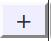
\includegraphics[height=13pt]{plus.jpg}}
to permanently add your job to the table.
Finally press \raisebox{-0.2\height}{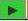
\includegraphics[height=13pt]{run.jpg}} to the right of your model setup file to create the model index itself.

\subsubsection{6. Check the log}
When the job is finished, check the log. You may view the log by pressing the link in the \lstinline!Last! column in the Auto tab table.
\begin{paperbox}{Model log}
  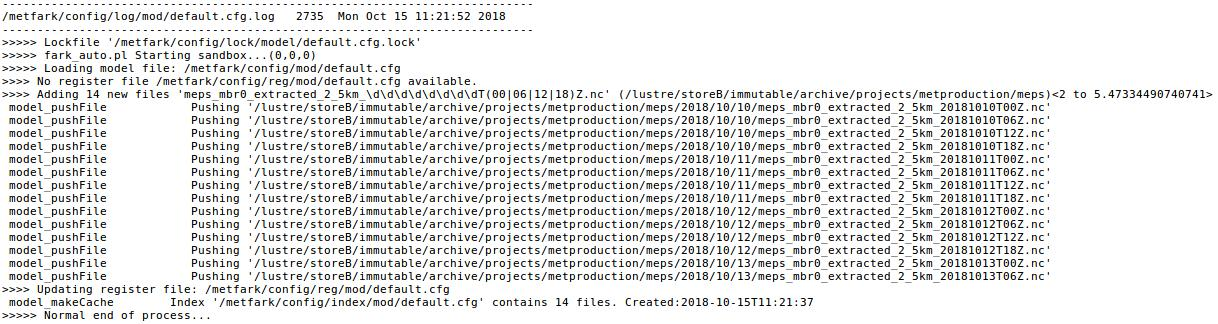
\includegraphics[width=\columnwidth]{modlog.jpg}
\end{paperbox}
The log lists the model-files added to the index together with the size and modification date of the index.
\begin{quotebox}
   The log of a successful run contains \lstinline!Normal end of process...!.
\end{quotebox}
Note that several processes flush output to the log, giving it a somewhat ``shuffled'' appearance.

\subsection{...create an observation index}
Change focus to the ``Observation'' tab. 
Creating the observation index setup is similar to creating the model index setup as indicated above.
However, editing the setup file is explained in some detail here.

After creating your new observation index setup, 
you may press \raisebox{-0.2\height}{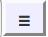
\includegraphics[height=13pt]{server.jpg}} next to
\lstinline!Obs file filter(regexp)! to select which observation file to scan.
\begin{paperbox}{BUFR type and Sub type}
  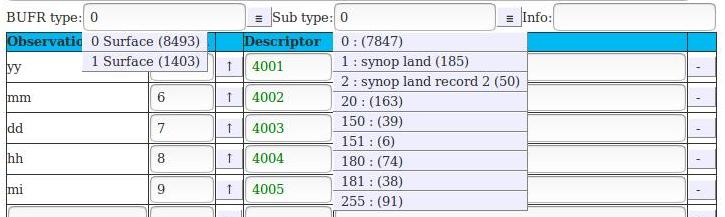
\includegraphics[width=\columnwidth]{how_obs.jpg}
\end{paperbox}
The \lstinline!BUFR type! and \lstinline!Sub type! alternatives are extracted from the scanned file,
along with their associated BUFR sequences.
Define the targets that you need in your observation index expression by entering values
in the bottom row of the \lstinline!observation targets! table, and by pressing the \raisebox{-0.2\height}{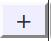
\includegraphics[height=13pt]{plus.jpg}} to the right.
You may remove a row by pressing  \raisebox{-0.2\height}{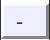
\includegraphics[height=13pt]{minus.jpg}} to the right of the respective row.
The values of the removed row are put in the bottom row.
When you are satisfied, press \raisebox{-0.2\height}{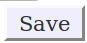
\includegraphics[height=13pt]{save.jpg}} to save your settings.

You may now add and run the job in the \lstinline!Auto tab! by pressing \raisebox{-0.2\height}{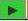
\includegraphics[height=13pt]{run.jpg}}. View the log-file by following the link in  the \lstinline!Last! column. The log lists the observation-files added to the index together with the size and modification date of the index.
\begin{paperbox}{Observation log}
  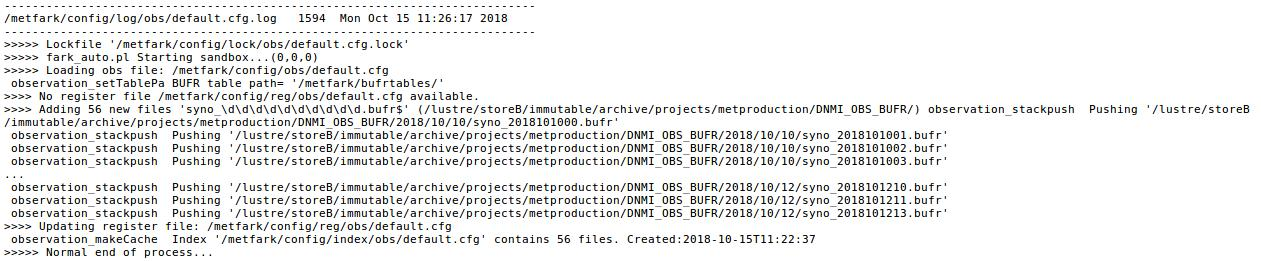
\includegraphics[width=\columnwidth]{obslog.jpg}
\end{paperbox}

\subsection{...create a colocation setup}
Change focus to the ``Colocation'' tab. 
Creating the colocation setup is similar to creating the model index setup as indicated above.

In the colocation setup you define model- and observation-targets, and how they should match.
Make sure you have scanned a model-file (\lstinline!Model tab!)
and observation-file  (\lstinline!Observation tab!)
so that model variables and observation BUFR sequences can be listed where relevant.

Add the model and observation targets needed to match an observation with the model, for instance
\lstinline!time!, \lstinline!latitude! and \lstinline!longitude!.
Add targets for the verification parameters, for instance \lstinline!pressure! and \lstinline!temperature!. Finally define the matching expressions.
When you are satisfied, press \raisebox{-0.2\height}{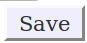
\includegraphics[height=13pt]{save.jpg}} to save your settings.

It is not recommended to run a colocation-job in the \lstinline!Auto tab! since this is an extremely slow process that generates an enormous amount of output.

\subsection{...create verification plots}
Before you can make verification plots, you must have
created a model and observation index, and a colocation {\em setup}.

Next you need to create a plot setup. Change focus to the ``Plot'' tab. 
Creating the plot setup is similar to creating the model index setup as indicated above. Remember to change the output-fields if you copied the plot setup.
When you are satisfied, press \raisebox{-0.2\height}{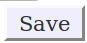
\includegraphics[height=13pt]{save.jpg}} to save your plot setup.

Next, switch to the \lstinline!Auto tab! and add your plot-job to the table.
To actually create the verification plots, press \raisebox{-0.2\height}{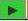
\includegraphics[height=13pt]{run.jpg}} next to your plot job and follow the link in the \lstinline!Last! column to see the log produced by the plot job.
\begin{paperbox}{Plot log}
  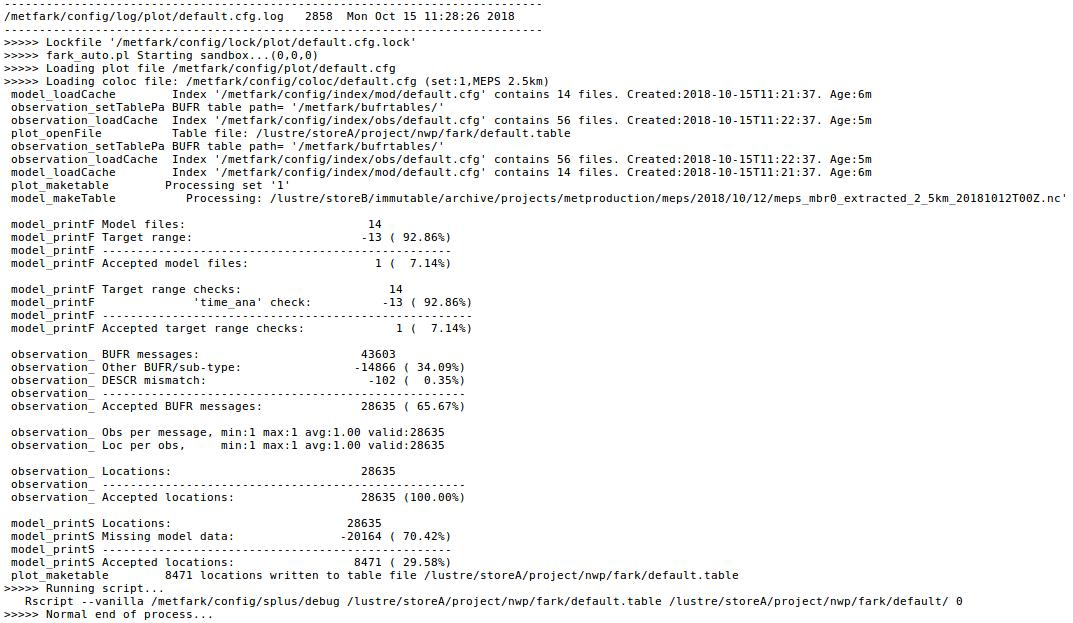
\includegraphics[width=\columnwidth]{plotlog.jpg}
\end{paperbox}

The plot log contains information on the indexes used, how many files they contained and when they were last modified.
The log also lists the model files that were processed, and a summary of how data was removed during the processing. This is a good place to start looking for missing data.
\begin{quotebox}
  Check if your indexes are up-to-date if your time-dependent filters have removed all data.
\end{quotebox}

The script command (usually listed at the end of the log), contains the root output directory for the verification results, which you specified in the \lstinline!Plot tab!. The next section shows some examples of verification plots that the ``synop'' verification script typically would place there.

\subsection{Examples}
Here are some examples of verification plots.
%that can be produced by FARK using the ``synop'' verification script. Verification plots are typically found under \lstinline!/lustre/storeA/project/nwp/fark!.

\begin{paperbox}{FF10m score}
  \centerline{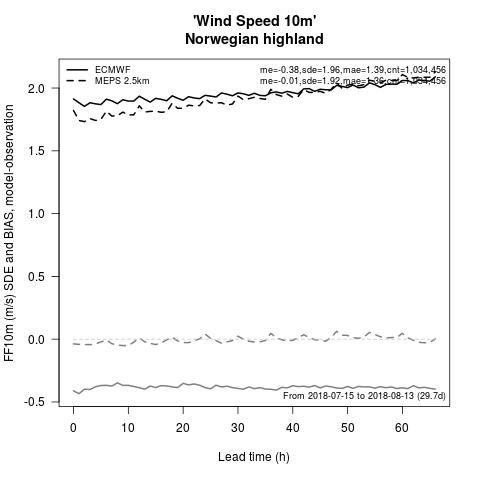
\includegraphics[width=0.8\columnwidth]{ff10m_score_hl.jpg}}
\end{paperbox}

\begin{paperbox}{FF10m vs MSLP}
  \centerline{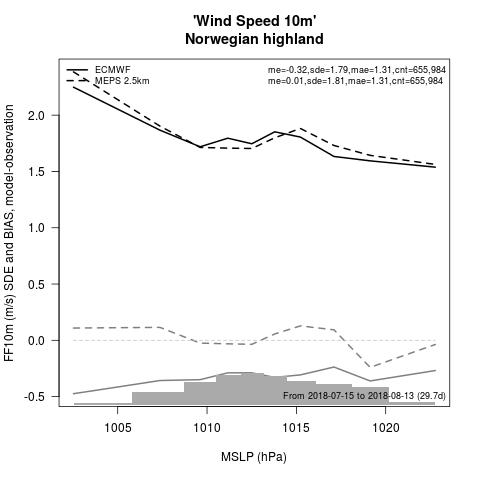
\includegraphics[width=0.8\columnwidth]{ff10m_mslp_hl.jpg}}
\end{paperbox}

\begin{paperbox}{FF10m profile}
  \centerline{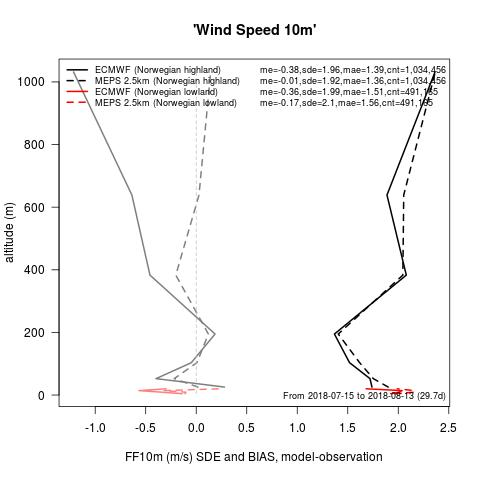
\includegraphics[width=0.75\columnwidth]{ff10m_prof.jpg}}
\end{paperbox}

\begin{paperbox}{FF10m SDE series}
  \centerline{\includegraphics[width=0.8\columnwidth]{ff10m_series_hl.jpg}}
\end{paperbox}

%\begin{paperbox}{FF10m MEAN series}
%  \centerline{\includegraphics[width=0.85\columnwidth]{ff10m_time_hl.jpg}}
%\end{paperbox}

%\begin{paperbox}{FF10m time series}
%  \centerline{\includegraphics[width=0.85\columnwidth]{ff10m_series_hl.jpg}}
%\end{paperbox}

%%\newpage
\hypertarget{appendix}{}
\section{Appendix}
\hypertarget{netcdf}{}
\subsection{NetCDF model files}
The NetCDF model files each contain a set of dimensions and variables, 
where each variable may have zero or more dimensions, for instance \lstinline!latitude(x,y)! where
\lstinline!x! and \lstinline!y! are dimensions. 
Note that some variables are accumulated, for instance \lstinline!precipitation_amount_acc(...,time)!. 
Rain rate is calculated by differentiating this variable with respect to time.

\hypertarget{bufr}{}
\subsection{BUFR observation files}
A BUFR observation file may contain many BUFR messages with different BUFR type and sub-type.
Each BUFR message may contain many observations of the same type, for instance SYNOP or TEMP. 
An observation may further contain many locations, for instance a radiosonde TEMP 
observation may contain data from many different heights in the atmosphere.


\hypertarget{sequence}{}
\subsection{BUFR sequence}
BUFR observations with the same BUFR type and sub-type use the same {\bf BUFR sequence}.
\begin{paperbox}{BUFR sequence example}
  \includegraphics[width=\columnwidth]{bufr1.jpg}
\end{paperbox}
The BUFR sequence contains a {\bf position}, {\bf descriptor} and {\bf value}
for each parameter in the observation.
The {\bf descriptor} is used to identify the observation parameter, for instance 
\lstinline!pressure! is identified by the descriptor \lstinline!7004!.
\hypertarget{delayed}{}
\subsection{Delayed replicator}
\begin{paperbox}{Delayed replicator}
  \includegraphics[width=\columnwidth]{bufr2.jpg}
\end{paperbox}

A BUFR sequence may contain a {\bf delayed replicator} (descriptor \lstinline!31001!), 
which will duplicate a sub-section of the BUFR sequence the specified number of times. 

\begin{quotebox}
  BUFR sequence positions after a {\bf delayed replicator} are not ``fixed''.
\end{quotebox}

\subsection{Performance}

Co-locating large amounts of data takes a lot of resources, and it is quite easy to
set up jobs that are not able to run successfully. Generating {\bf table files}
does not usually require too much memory but can take much processing time.
However the {\bf plotting script} will typically not be able to process a {\bf table file} with 
more than 10 million entries without running out of memory (on Ares). 
This corresponds to 20 days of verification for northern Europe.
Although FARK has all the features necessary for a full verification of
operational forecast ensemble data using radiosonde data, this is option is
probably not realistic from a computer resource perspective.




% End document
\end{document}

